\chapter{Method}


Several hypotheses were tested in this work.
Section \ref{architecture} describes the technical set up required for running all these experiments and deploying the model to production before delving into the specific experiments and their evaluation methods in sections [ref].

\hfill \break \noindent
The experiments were conducted in four distinct stages:

 \begin{itemize}
   \item Training a baseline model on the rule-based labels to get a sense of the difficulty of this problem. Since there is no fundamental difference in the way this model was  trained and evaluated compared to the other classifiers, this is described in section \ref{exp_models} with the others. After this step, in ground truth dataset was obtained.
   \item Training the independent classifiers to determine best performers (\ref{exp_models}).
   \item Training an ensemble of the independent classifiers (\ref{exp_ensembling}).
   \item Training up to 10 iterations of active learning on the strong predictor (\ref{exp_al}).
 \end{itemize}

\section{System Architecture}
\label{architecture}

 The following technologies were used to build the system which had to interact with existing services  at the client company:

\begin{itemize}
  \item ElasticSearch - a NoSQL database with powerful full-text search and querying capabilities.
  \item RabbitMQ - a message queue, used for transferring data among our microservices (using the Logstash adapter, that can read from and write to (among other things) ElasticSearch and RabbitMQ).
  \item MySQL - a relational database.
  \item Flask - a simple backend web framework for Python.
  \item Node.js - a JacaScript backend web framework.
  \item React.js - a JavaScript front-end framework for JavaScript.
  \item Redux - a framework for persisting user interface (UI) state and application data in single page applications.
  \item Google Cloud Storage (GCS) - Google Cloud Platform (GCP) object storage similar to Amazon S3.
  \item Apache Beam - a data processing engine akin akin to Apache Spark and Apache Flink.
  \item Dataflow - a GCP service for executing Apache Beam workloads.
  \item TensorFlow - ML framework for Python, capable of defining many kinds of models as a computation graph, and executing this graph locally or in a distributed manner.
  \item ML Engine - a GCP service for running TensorFlow models (training, hyperparameter tuning, inference).
  \item Apache Airflow - a Python framework for defining workflows of long-running tasks and dependencies between these tasks.
\end{itemize}

All the product data was read from and written to ElasticSearch.
was used for storing information about categories, but this was transitioned over to ElasticSearch
was used for building the initial application for displaying the results of the baseline (predictions, averaged and per-class evaluation metrics). The front end was built with React.
the web application was later rewritten by another employee of the client company, so  that he could implement the more labour-intensive  passing a language is more familiar with.

\begin{figure}
  \hspace*{-0.2\textwidth}
  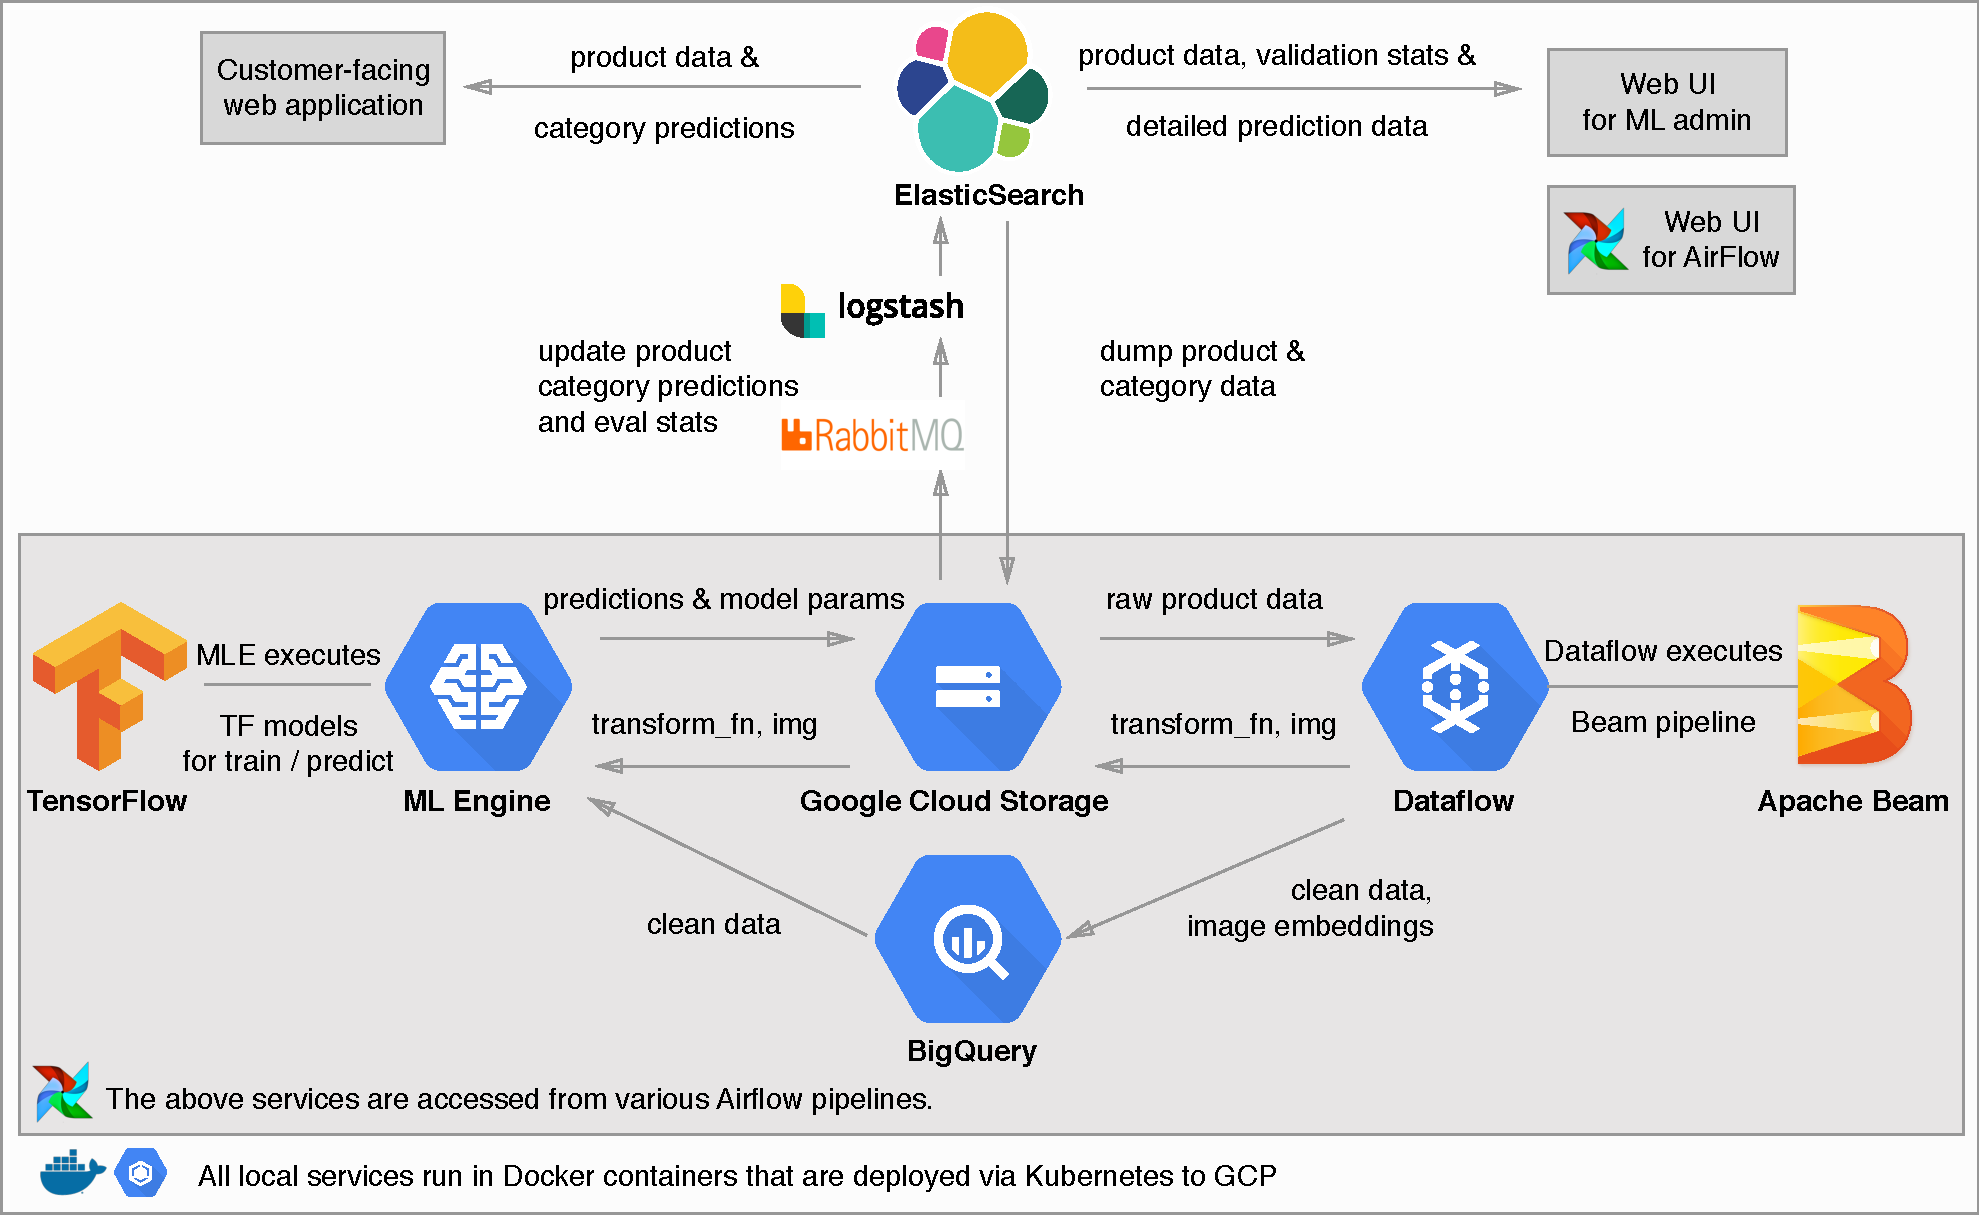
\includegraphics[width=1.4\textwidth]{diagrams/architecture}
  \caption{High-level system architecture of the ML pipeline}
  \label{arch_diagram}
\end{figure}


\section{Experiments}
\subsection{Independent Models}
\label{exp_models}

\subsection{Ensembling}
\label{exp_ensembling}

\subsection{Active Learning}
\label{exp_al}



\section{Evaluation}
\label{evaluation}

At the beginning of running all these experiments, the dataset was divided into development and test set (90/10\%).
The development set was used for


 we can evaluate the performance of the model on three types of datasets:

\begin{itemize}
  \item the test or validation set as labelled by the rule-based system (referred to as ``rule-based test/validation set''),
  \item the ground truth dataset gathered  before running most experiments,
  \item
\end{itemize}
